\documentclass[crop,tikz]{standalone}
\usetikzlibrary{shapes}
\usetikzlibrary{arrows}
\usetikzlibrary{positioning}

\begin{document}
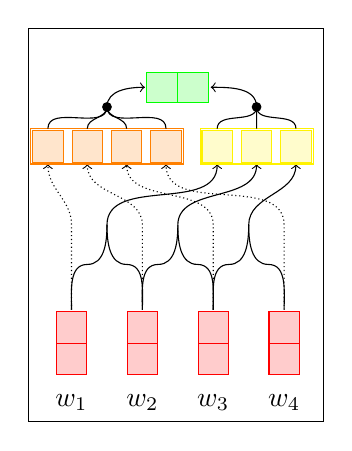
\begin{tikzpicture}[
  hid/.style 2 args={
    rectangle split,
    draw=#2,
    rectangle split parts=#1,
    fill=#2!20,
    outer sep=.25mm},
  mlp/.style 2 args={
    rectangle split,
    rectangle split horizontal,
    draw=#2,
    rectangle split parts=#1,
    fill=#2!20,
    outer sep=.25mm}
]

 % Comment out this line to remove border.
 \draw[draw=black] (0, 5) rectangle (3.75, 0);

 \foreach \step in {1,...,4} {
   \node (i\step) at (.9*\step -.35, .25) {$w_\step$};
   \node[hid={2}{red}] (e\step) at (.9*\step - .35, 1) {};    
 }
 
 \node[mlp={2}{green}] (s) at (.9 * 2.5 - .35, 4.25) {};
 
 
 \foreach \last/\next in {1/2,2/3,3/4} {
  \node[hid={1}{yellow}] (a2\last) at (.5 * \last + 1.9, 3.5) {};
  \draw[->] (e\last.north) to [out=90,in=180] (.9 * \last + .2 - .35, 2) 
  to [out=0,in=270] (.9 * \last  + .45 - .35, 2.5) 
  to [out=90,in=270](a2\last.south);
  \draw[-] (e\next.north) to [out=90,in=0] (.9 * \next  - .2 - .35, 2) 
    to [out=180,in=270] (.9 * \last + .45 - .35, 2.5);
 }

 \foreach \step in {1,...,4} {
  
  \node[hid={1}{orange}] (a1\step) at (.5 * \step -.25, 3.5) {};
  \draw[->,densely dotted] (e\step.north) to (.9 * \step - .35, 2.5) 
  to [out=90,in=270] (a1\step.south) {};
 }

 \draw[draw=orange] (a11.north west) rectangle (a14.south east);
 \draw[draw=yellow] (a21.north west) rectangle (a23.south east);
 \draw[-] (a21.north) to [out=90,in=270] (2 * .5 + 1.9, 4);
 \draw[-] (a23.north) to [out=90,in=270] (2 * .5 + 1.9, 4);
 \draw[->] (a22.north) to [out=90,in=270] (2 * .5 + 1.9, 4) 
    to [out=90,in=0] (s.east);
 \node[circle,fill,inner sep=1.25pt] (t) at (2 * .5 + 1.9, 4) {};


 \draw[-] (a11.north) to [out=90,in=270] (2.5 * .5 -.25, 4);
 \draw[-] (a12.north) to [out=90,in=270] (2.5 * .5 -.25, 4);
 \draw[-] (a13.north) to [out=90,in=270] (2.5 * .5 -.25, 4);
 \draw[-] (a14.north) to [out=90,in=270] (2.5 * .5 -.25, 4);
 \draw[->] (2.5 *.5 -.25, 4) to [out=90,in=180] (s.west);
 \node[circle,fill,inner sep=1.25pt] (t) at (2.5 * .5 -.25, 4) {};


%    to [out=0,in=90] (.9 * 2.5 - .35, 2.5) to (s.south);
% \draw[-] (e4.north) to [out=90,in=0] (.9 * 3.5 - .35, 2) 
%    to (.9 * 2.75 - .35, 2)
%    to [out=180,in=90] (.9 * 2.5 - .35, 2.5) to (s.south);

 %\draw[-] (e3.north) to [out=90,in=0] (.9 * 2.75 - .35, 2) ;
 %\draw[-] (e2.north) to [out=90,in=180] (.9 * 2.25 - .35, 2) ;

%   \node[circle,fill,inner sep=1.25pt] (t) at (.9*2.5 - .35, 2.75) {};
%   \node[white] (p) at (.9*2.5 - .35, 2.75) {\scalebox{.4}{\textbf{+}}};
 
\end{tikzpicture}
\end{document}
